\section{Methodology}

In order to investigate the current state of health of the Go
eco-system, you need to compile a lot of Go packages. You also need to
do some statistics on them.

In order to more easily get multiple modules, at various versions,
compiled through an instrumented build environment, the author built
an environment consisting of a validator (custom Go code), Athens
(pre-existing Docker container), and an instrumented build environment
(custom Python, in a Docker container).

\begin{figure}[ht]
  \label{fig:architecture}
  \caption{Rough system architecture, depicting JSON requests, module requests and execution with different arrows}
  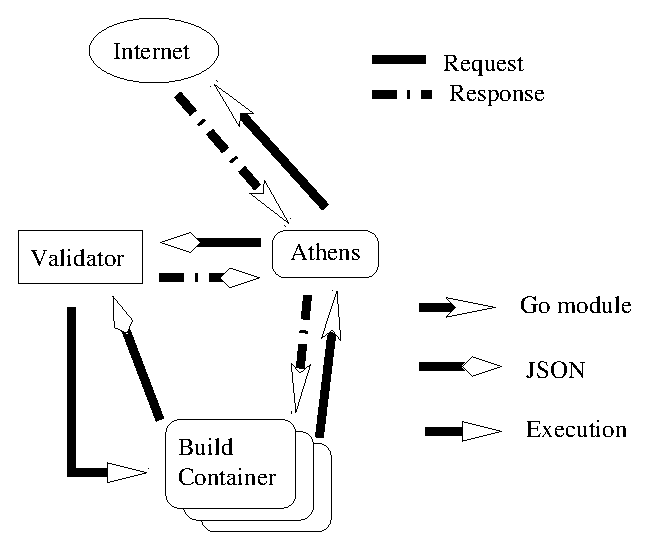
\includegraphics{architecture.eps}
\end{figure}


The validator considers all module/version tuples as valid. If the
specific module/version tuple has not been seen before, a build of
that is started\footnote{Technically, placed in a build queue}. The
validator limits builds to at most five concurrent ones, this is to
preserve some responsitivity on the test machine. It is possible to
increase the build parallelism by having more ``build workers''. The
number of build workers is set at compile time.

The custom build environment then reports back some general statistics
(did ``go mod download'' work, could we list all targets in the
downloaded code, did all builds succeed, did all tests succeed, how
many build/test targets, did go vet pass\footnote{This is a new test
  for this report}, and (on failure) what build/test targets
failed). The build environment is set up to use the Athens instance as
its GOPROXY, making it much easier to get a wide spectrum of code
scanned, as all transitive dependencies from the seed modules end up
being processed.

The validator periodically writes its current data set to disk. There
is also a web endpoint that triggers a save when accessed. The
validator will only create a new save file if there's been any
changes\footnote{Note, a ``change'' really means ``there has been
  build results reported'', in practice this is enough in the early
  stages of data gathering.}  since the last save.

To seed the scan, a few packages were manually started within the
build container, using the same environment as that set up by the
validator. For more details, see the section on seed packages.

The source code for the tabulator, the validation web-hook framework
and the build instrumentation can be found at
https://github.com/vatine/gochecker/ .


\subsection{Methodology changes for the latest report}

\subsubsection{Downloads}

Due to various changes in how Go modules are fetched, the wrapper has
been intrsumented to report ``module that can be downloaded, but has
one or more immediate missing dependencies'' as ``download succeeded,
build error'', whereas in previous versions that may have been
reported as a download error.

\subsubsection{Data cleaning}

The latest report also has a ``data cleaning'' component, that deletes
names tha can definitely not be module names (bare host names, github
users or organisations, golang.org/x and a few others, specific
details will be in source code). Only module-version tuples flagged as
``download failed'' are eligible for being cleaned from the data set.
